% Do not change the options here
\documentclass[bsc,frontabs,parskip,deptreport]{infthesis}

\usepackage{graphicx}
\usepackage[%  
    colorlinks=true,
    pdfborder={0 0 0},
    linkcolor=black,
    citecolor=blue
]{hyperref}


\begin{document}
\begin{preliminary}
\title{A Zoom filter for applause and laughter}

\author{Lasse Wolter}

% to choose your course
% please un-comment just one of the following
%\course{Artificial Intelligence}
\course{Artificial Intelligence and Computer Science}
%\course{Artificial Intelligence and Mathematics}
%\course{Artificial Intelligence and Software Engineering}
%\course{Artificial Intelligence with Management}
%\course{Cognitive Science}
%\course{Computer Science}
%\course{Computer Science and Management Science}
%\course{Computer Science and Mathematics}
%\course{Computer Science and Physics}
%\course{Computer Science with Management}
%\course{Software Engineering}
%\course{Software Engineering with Management}

\project{4th Year Project Report}

\date{\today}

\abstract{j

% This skeleton demonstrates how to use the \texttt{infthesis} style for
% undergraduate dissertations in the School of Informatics. It also emphasises the
% page limit, and that you must not deviate from the required style.
% The file \texttt{skeleton.tex} generates this document and can be used as a
% starting point for your thesis. The abstract should summarise your report and
% fit in the space on the first page.
}

\maketitle

\section*{Acknowledgements}


\tableofcontents
\end{preliminary}


% The preliminary material of your report should contain:
% \begin{itemize}
% \item
% The title page.
% \item
% An abstract page.
% \item
% Optionally an acknowledgements page.
% \item
% The table of contents.
% \end{itemize}

\chapter{Introduction}

Achievements
\begin{enumerate}
  \item Evaluation of existing laughter detection model on the whole ICSI meeting corpus
  \item Investigation of bad performance of this model on ICSI corpus
  \item Retrain model on ICSI corpus
\end{enumerate}

\chapter{Background} \label{cha:bg}
Automatic applause and laughter detection isn't a new idea. Nevertheless, the research in these two areas is usually done separately. There are a few papers which cover both, one of the most popular ones being from Cai et. al \cite{cai2003highlight} who used sound effect detection - which included laughter and applause - for video summarisation and highlight extraction.
Apart from this and a few other papers most research only covers one of the two domains, either applause or laughter. Thus, we split the review of existing research into the following sections:
\begin{enumerate}
  \item Laughter Detection
  \item Applause Detection
  \item Evaluation Metrics 
\end{enumerate}


\section{Laughter Detection} \label{sec:bg-laughter}
The investigation of the acoustic features of laughter reaches back three decades \cite{bickley1992acoustic}.
In the early 2000s, the first attempts of laughter detection in conversational speech classified presegmented audio data \cite{kennedy2004laughter, truong2005automatic}. These models could only decide whether laughter occurred within in a given segment. The determination of segment boundaries of laughter events wasn't considered. 
Corpora used in these papers include the development data from the 2004 Spring NIST Rich Transcription Evaluation \cite{ldcnistcorpus}, the Dutch CGN corpus \cite{oostdijk2000spoken} as well as the ICSI Meeting Recorder corpus \cite{morgan2001meeting}. 

Two examples of such classification of presegmented audio data were presented by Kenney and Ellis \cite{kennedy2004laughter} and Truong and Van Leeuwen \cite{truong2005automatic}. 
Even though both models classified presegmented audio there were some significant differences. 
Firstly, the definition of laughter and the motivation behind the research differed.
While Kennedy and Ellis define laughter events as 'points in the meeting where more than one person laughs', Truong and Van Leeuwen considered one person laughing as a laughter event.
Kennedy and Ellis didn't specify a particular motivation whereas Truong and Van Leeuwen's long-term goal was the investigation of 'paralinguistic events' - laughter being one of them - to classify the speaker's emotional state.   

Secondly, there was a difference between the best performing features and predictors.  
Kennedy and Ellis \cite{kennedy2004laughter} got the best results using Mel Frequency Cepstral Coefficients (MFCCs) as features and a Support Vector Machine (SVM) for decision making. 
In contrast, Truong and Van Leeuwen \cite{truong2005automatic} used Perceptual Linear Prediction (PLP) features with Gaussian Mixture Models (GMM) for classification. 

Truong and Leeuwen \cite{truong2007automatic} continued their research and stated that spectral features alone (such as PLP and MFCCs) can be used to discriminate between laughter and speech but a significant improvement can be achieved when using prosodic features - features relating rhythm and intonation.

In 2006, Knox and Mirghafori \cite{knox2006automatic} were the first to do laughter recognition without the need for presegmented audio data.  
They worked with the Bmr-subset of the ICSI Meeting corpus \cite{morgan2001meeting} to be able to compare their results to previous research done on this dataset \cite{kennedy2004laughter, truong2005automatic, truong2007automatic}.

Their goal was to obtain accurate interval boundaries of laughter segments.
One limiting factor for the precision of these boundaries is the frame size. 
When Knox and Mirghafori first experimented with SVMs similar to Kennedy and Ellis \cite{kennedy2004laughter}, they realised that the time to compute the features and train the SVM increased significantly with decreasing frame size. 
This is due to the fact that aggregate statistics need to be calculated and stored for each frame of training data.  
On the contrary, a neural network trained with features from a context window can directly use the features of each frame without aggregating them.  

To obtain frame-level training labels for the ICSI dataset Knox and Mirghafori first removed all segments that contained both speech and laughter under a single start and end time because the laughter specific interval boundaries couldn't be identified in those segments. 
The remaining audio data could be accurately separated into laughter and non-laughter segments which were then divided into 10ms frames and labeled accordingly.

The model was trained to classify each 10ms frame using a window of 75 frames around the target frame - 37 before and 37 after the frame (\ref{fig:know_window}).
This way an accurate prediction of laughter boundaries of up to 10ms was possible. 
The features investigated by Knox and Mirghafori are MFCCs, AC PEAK, F0 and RMS as well as their corresponding delta and delta-delta features.
They first trained four separate neural networks each one taking one of the mentioned features as input.
Afterwards they combined the different models by using their output as input for another, smaller neural network.
The best results were obtained by combining the outputs of three NN-systems which used delta MFCCs, AC PEAK and F0 as features, respectively.
By training and evaluating separate neural networks for each type of feature first, Knox and Mirghafori observed that MFCCs have the most discriminative power which aligns with prior research by Kennedy and Ellis \cite{kennedy2004laughter}.

\begin{figure}[htp]
    \centering
    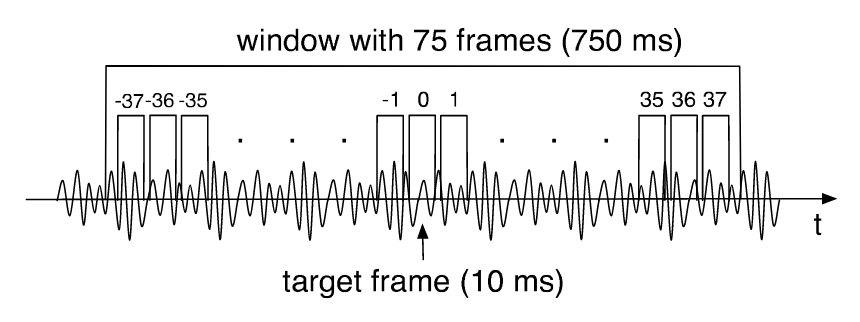
\includegraphics[width=10cm]{imgs/Knox_window.png}
    \caption{Frame window used by Knox and Mirghafori}
    \label{fig:know_window}
\end{figure}

A survey from 2016 \cite{cosentino2016quantitative} investigates research on laughter and laughter detection in different fields up to that time.
This survey covers different detection methods using visual, acoustic and sensory data.
For this thesis laughter detection using solely acoustic features is the most relevant. Consentino et al. \cite{cosentino2016quantitative} find that in such cases best performance was obtained using MFCCs and PLPs as features and combining the resulting classifier with ones that also use prosodic features.
This aligns with findings from prior research \cite{truong2007automatic, knox2006automatic}.

More recent research by Gillick et al. \cite{gillick2021robust} finds that features learned from spectrograms using deep convolutional networks outperform previous approaches based on MFCCs.
Their hypothesis was that models using MFCCs are more prone to pick up surface level characteristics of sound and thus, will be more sensitive to variations like background noise.
Gillick et al. expected that features learned using a CNN are more representative of the actual laughter and thus, more robust to different environments. 
Their results show that a model using features learned by a CNN architecture outperforms the conventional approach using MFCCs. 


\section{Applause}
The following review is less exhaustive compared to the review on laughter detection.
This is due to the fact that we decided to focus on laughter detection for now and possibly add applause detection afterwards.
More information on this decision can be found (TODO: Link to corresponding section).

As mentioned at the beginning of this chapter, in 2003 Cai et al. \cite{cai2003highlight} worked on the detection of sound events, including but not limited to applause.
They used perceptual features and MFFCs as features, Hidden Markov Models (HMM) and Gaussian Mixture models (GMM) to model sound and log likelihood for decision making.
Cai et al. evaluated their system on a testing set consisting of 2 hours of video material from different programs.
For applause specifically they achieved a precision of 87.37\% and a recall of 92.00\%.

In contrast, Uhle \cite{uhle2011applause} used MFCCs and low-level descriptors (LLD) to represent sound and passed these features to an MLP or an SVM for classification.
The difference between MLP and SVM classifier were rather small.
Uhle worked with a relatively small dataset consisting of 210 snippets of 9-30s length. This equates to a total length between 31.5 min and 105 min.
On a rather small test (10\% of this dataset) Uhle achieved an accuracy of 95\% with a precision 96.51\% and recall of 97.65\%.

A less complex approach for applause detection was presented by Li et al. \cite{li2009characteristics}.
They used a manually created 4-layer decision tree to classify a given sound input as applause or not-applause.
Testing their model on 50 hours of meeting speech containing 500 applause segments ranging from 0.8 to 36s they were able to retrieve 491 of the 500 applause segments while incorrectly retrieving 38 non-applause segments.
This equates to a recall of 98.2\% and a precision of 92.82\%. Li et al. also compared their less complex model to the HMM model proposed by Cai et al.\cite{cai2003highlight} and outperformed it while using less computational time.

Manoj et al. \cite{manoj2011novel} proposed another approach based on manually created decision trees. They also compared it to a more complex model similar to the one proposed by Cai et al. \cite{cai2003highlight} - with the difference that this model only used GMMs, no HMMs.
Even though the decision tree stages were different to Li et al. \cite{li2009characteristics} the findings are similar. The decision tree outperforms the more complex method using MFCCs and GMMs.  

\section{Evaluation metrics} \label{theory}
still to be written


\chapter{tbd} 

\section{Model and data selection}\label{sec:model-and-data}
After having done the initial research we decided to focus solely on laughter detection. 
There are two main reasons for this, type of previous research and open source code available.  
As mentioned in the background chapter (\ref{cha:bg}) most research in the field of laughter and applause detection is done separately. 
Thus, implementing a detection algorithm from existing research requires merging different models. 
For a combined model to work it is essential that a good understanding of each domain is already present.
We decided that this is most easily attained by focusing on one domain first. 
We chose to focus on laughter instead of applause due to the second reason mentioned above.
There was an open-source repository available which showcased an existing state-of-the-art laughter detection algorithm.
In fact, the corresponding paper by Gillick et al. \cite{gillick2021robust} was just published a month before this project started.


To investigate how this existing model might perform in our considered domain, namely single-person audio recordings - as it is the standard in video conferences - we decided to evaluate it on the ICSI meeting corpus \cite{morgan2001meeting}. 
We initially considered the use of Audio Set \cite{googleaudioset} as a possible evaluation corpus. After some discussion we discarded this idea because of a mismatch with the domain for our project. Audio Set was built by extracting 10s audio segments from Youtube videos and assigning it to one a set of classes. Laughter is one of the classes considered. Nevertheless, the domain of Youtube videos varies drastrically. It can be a recording of someone laughing in a silent environment inside a room or someone laughing in a very noisy environment outside. This variety of environments might help for generalising laughter detection but isn't suitable for our project where we focus on laughter detection in a relatively quiet environment with audio being recorded individually for every single person.
In contrast, the ICSI corpus was a good match to our domain as it solely consists of meeting speech recorded with both close-distance and table-top microphones. 
We only make use of the close-distance microphone recordings which capture the audio of a single meeting participant.
Laughter occurrences aren't reported by class assignment as in Audio Set. The ICSI corpus provides transcriptions for all its participants containing speech as well as \texttt{Vocal} and \texttt{NonVocal} tags for sounds like microphone noise and laughter. 

Transcriptions are split into segments denoted by a start and end time. Consequently laughter segments cannot be precisely identified if they occur in one segments next to speech. Thus, laughter annotations cannot be considered strongly labeled data. Nevertheless it is possible to get strongly labeled annotations by only using those laughter segments that appear in a transcription segments by itself (see \ref{sec:model-eval}).
Another reason for choosing the ICSI database is it is size - about 75 hours.
Even after filtering for laughter segments that occur on their own, there are still 8420 snippets with an accumulated duration of 3.9h. 
We considered this a reasonable size to do evaluation on. 


\section{Model Evaluation} \label{sec:model-eval}
The first part of evaluation was to filter out the segments that only contain laughter. As mentioned in \ref{sec:model-and-data} this was required to get strongly labeled data. Strongly labeled training data is key for our project as we are trying to accurately determine the boundaries of laughter segments. 
It is not enough to simply determine if a certain interval contains laughter or not as this won't help in determining accurate segment boundaries. 
The process of filtering for snippets only containing laughter is similar to Knox and Mirghafori's approach to obtain frame-level training data \cite{knox2006automatic} (\ref{sec:bg-laughter}). 
Another approach would have been to use an ASR model to align transcriptions with audio. Considering the sufficient amount of laughter segments attained with the simple approach presented above, this more complex and more time consuming approach wasn't necessary. For future projects this might be a useful approach to gain more accurate training/testing data. 
In contrast to some of the research presented in the background chapter which only used a subset of the ICSI corpus we used the whole dataset for evaluation. We ran the pre-trained detection model by Gillick et al. with four different thresholds for each channel of the 75 meetings - a total of 468 audio tracks. 
Precision and recall for those 1872 experiments can be found in table (TODO).
A precision-recall curve was plotted (fig:TODO). The precision recall curve has the expected shape but visualises the main problem. The maximum recall achieved is 31.53\%. We expected that a low threshold like 0.2 would yield low precision. Getting such a low recall, however, was surprising. 
Initially we thought that there might be something wrong with our evaluation method. After some discussion we realised that the discarded laughter occurrences to get strongly labeled data weren't discarded from the predictions. This meant that the model could classify a laughter occurrence correctly but the evaluation method would consider it as false because this laughter occurrence was discarded pre-evaluation. This discrepancy in preprocessing was easily fixed and as one would expect the precision was significantly (fig: TODO). Nevertheless, the recall remained almost unchanged. 

To make these results more tangible we did a theoretical experiment. What would happen is such is system was deployed? The results of this practical experiment can be seen in table TODO. 
Considering any of the four possible systems - with different thresholds each - it is aparent that such a system would be entirely unusable. We'll briefly examine the two extreme cases. If the threshold was really low, e.g. 0.2, not roughly TODO minutes of TODO minutes laughter would be correctly retrieved. Despite this being a not even half of the laughter events that actually occurred we also got about TODO minutes of noise.  
On the other hand, choosing a high threshold, e.g. 0.8, yields very high precision and thus, no noise is transmitted. Even though no noise is retrieved we merely retrieve TODO minutes of laughter in a meeting of TODO minutes. With such a low percentage of retrieved laughter events there is not much difference to entirely muting yourself. 

A possible reason for such a bad performance on the ICSI corpus is a data mismatch between training and evaluation data. The pre-trained model by Gillick et al. \cite{gillick2021robust} was trained on the Switchboard corpus \cite{switchboard-corpus}. The Switchboard corpus records telephone conversations between two participants at a sample rate of 8000hz. The ICSI corpus records meeting speech of multiple participants at a sample rate of 16000hz. The Switchboard dataset has one audio track containing all audio whereas the ICSI corpus has a separate audio track for each participant.  
TODO: possible other differences?
These differences suggest that a model trained on one of these corpora might not perform well on the other one. 
TODO: How does this tie in with Gillick et al.'s statement that they tried to create a detection algorithm that performs better on noisy data? How do they define "work well"? Did this cause the model to perform worse on quiet data?
In response to this finding we decided to retrain the model on the ICSI dataset. 

\chapter{tbd}
\section{Retraining the model}
The first approach was to adapt the code that Gillick et al. used and published. After investigating their code, I created a diagram of their data-pipeline (TODO: add figure). 
I created a similar one for our project and after consultation with my supervisors decided that the hash-map containing the preloaded audio could be neglected for now. 

After looking at their code in more detail,  
I realised that the code wasn't very concise and didn't seem to adhere to current standards of pytorch programs. 
For example, they used a manual counter for training steps and triggered a new training phase with 1 epoch each time instead of using this training function and passing more than one epoch as argument. 
Design decisions like this make the code harder to read and harder to debug. 
Another realisation was that Gillick et al. programmed lots of augmentation and transformation functions themselves instead of using existing implementations from libraries like pytorchaudio. 
Programming functions for turning audio files into spectrograms and padding/truncating audio files to a certain length themselves, makes the code unnecessary long and introduces risk for errors. In my opinion using existing and exhaustively tested functions from a popular framework like pytorchaudio is better in terms of readability and efficiency of the code.
My supervisor doesn't have much experience with pytorch but agreed that he doesn't consider the code as well written.

Despite the concerns about Gillick et al.'s code mentioned above, I decided to try to adapt their code for two main reasons. 
Firstly, I haven't worked on an ML project of this scale before and writing training and inference code from scratch seemed somewhat daunting to me. I didn't think that doing that would make things easier as I trusted that the code that Gillick et al. published should be usable as they have used it for a paper they published \cite{gillick2021robust}. 
Secondly, I thought that using their code and just doing minimal adjustments to load the ICSI corpus instead of the switchboard corpus would allow for an easier comparison between the two. If I wrote the code from scratch I'd have to make sure that all the preprocessing and model parameters are sufficiently similar to state the difference of changing the training data. 

After working on adapting the training code for about a week I ran into a major problem regarding the time it takes to train the model. I merely managed to train around 30 batches of audio, each consisting of 32 audio tracks, in 2 hours. This couldn't be right as the audio samples loaded from these audio tracks were only 1 second segments. This equates to 8s of processing time per 1s sample.
This is significantly slower than the evaluation on a CPU-only machine. TODO:cite rtf table

After some further investigation I realised that it's the data-loading that takes so long. I ran some experiments to check how long it takes to load the data (TODO: add exp data) and found that it's unacceptably slow. 

I discussed these results with my second supervisor and he suggested that it might be due to the different recording length of the switchboard dataset. According to LDC data (TODO link?) the switchboard dataset contains 2400 recordings and a total of approximately 260 hours of speech. This equals an average recroding length of roughly 8 mintues. Compared to the 52 minutes average (TODO check number) of the ICSI recording corpus this is a significant difference. 
As mentioned before I hadn't done the preloading of audio data like Gillick et al.. I thought about adding that to the pipeline but realised that it doesn't work because not all of the data can be loaded into memory. I'm not sure how Gillick et al. did it for the switchboard dataset. I thought about splitting the training data into subsets and preloading those one by one. This would have meant that the dataloader should only load data from a certain subset and switch to a new subset once this subset has been exhausted. 
For me this seemed to complicate the code even more and after consultation with my second supervisor I decided to rewrite the data-loader from scratch. 

My second supervisor suggested to possibly use lhotse (TODO: add link) which seemed promising so I decided to try that. 







\chapter{Other}
\section{Privacy Concerns}\label{privacy-concerns}
People might have privacy concerns if their visual input is used for classification.
Additionally, in video meetings and conferences people often turn off their video input.
Consentino et al. \cite{cosentino2016quantitative}  mention the privacy implications of video input and raise the same concern for audio input.
Thus, they suggest the use of individual wearable sensors to address these concerns.
For our project this approach isn't feasible and further, wearable devices might be quite intrusive.
In our system people can opt-out of using the laughter-detection feature at any time.
That way people stay in control of their own privacy.

\bibliographystyle{plain}
\bibliography{mybibfile}

%% You can include appendices like this:
% \appendix
%
% \chapter{First appendix}
%
% \section{First section}
%
% Markers do not have to consider appendices. Make sure that your contributions
% are made clear in the main body of the dissertation (within the page limit).

\end{document}
